% Nội dung chuyển từ báo cáo Word hiện tại.
\majorheading{MỞ ĐẦU}

Đặc điểm đất và điều kiện khí hậu là những thông tin cần xem xét khi lựa chọn cây trồng. Đề tài sử dụng dữ liệu về dinh dưỡng đất, pH, nhiệt độ, độ ẩm và lượng mưa để nghiên cứu bài toán phân loại cây trồng. Kết quả được đánh giá trong phạm vi bộ dữ liệu, phục vụ việc tìm hiểu phương pháp học máy.


Mục tiêu nghiên cứu là xác định đầu vào và đầu ra của bài toán, phân tích đặc điểm dữ liệu, xây dựng quy trình tiền xử lý và lựa chọn chiến lược đánh giá phù hợp. Dữ liệu được khảo sát về phân bố, quan hệ giữa các biến, giá trị thiếu, bản ghi trùng và dấu hiệu ngoại lai.


Báo cáo gồm ba chương. Chương 1 trình bày cơ sở lý thuyết học máy. Chương 2 trình bày bài toán, dữ liệu và phương pháp nghiên cứu. Chương 3 trình bày thử nghiệm và đánh giá.


\majorheading{CHƯƠNG 1. CƠ SỞ LÝ THUYẾT}

\section{1.1. Tổng quan về học máy}

\subsection{1.1.1. Khái niệm và vị trí của học máy}

Học máy là lĩnh vực nghiên cứu cách để máy tính học quy luật từ dữ liệu. Người xây dựng cung cấp các ví dụ, xác định nhiệm vụ và chọn cách đánh giá. Từ đó, máy tính tìm một quy tắc để xử lý những trường hợp tương tự. Chẳng hạn, từ các thư điện tử đã được gắn nhãn, chương trình có thể học cách phân biệt thư rác với thư thông thường. Mục đích của việc học là đưa ra kết quả phù hợp cho dữ liệu mới, thay vì chỉ ghi nhớ các ví dụ đã có.


Một nhiệm vụ học máy gồm ba thành phần: công việc cần thực hiện, dữ liệu hoặc kinh nghiệm dùng để học và thước đo kết quả. Với nhận diện thư rác, công việc là phân loại thư, dữ liệu học là các thư đã có nhãn, còn thước đo có thể là tỷ lệ phân loại đúng. Với dự đoán một đại lượng, công việc và thước đo sẽ thay đổi cho phù hợp. Xác định rõ ba thành phần này giúp người thực hiện biết cần thu thập dữ liệu gì và dựa vào đâu để nhận xét kết quả.


Trong lập trình theo quy tắc, người lập trình viết sẵn các điều kiện xử lý. Trong học máy, chương trình tìm quan hệ giữa đầu vào và đầu ra từ những ví dụ được cung cấp. Con người vẫn quyết định cách thu thập dữ liệu, ý nghĩa của nhãn và mức sai sót có thể chấp nhận. Vì vậy, kết quả học phụ thuộc nhiều vào chất lượng dữ liệu và cách đặt bài toán. Khi dữ liệu sử dụng khác với dữ liệu huấn luyện, chương trình có thể vẫn chạy bình thường nhưng dự đoán kém chính xác. Việc đánh giá cần kiểm tra cả mã nguồn lẫn kết quả trên dữ liệu chưa dùng để học [1].


Học máy là một hướng tiếp cận trong trí tuệ nhân tạo và có quan hệ chặt chẽ với thống kê, tối ưu hóa và khoa học máy tính. Thống kê cung cấp ngôn ngữ để mô tả biến thiên và suy luận từ mẫu; tối ưu hóa hỗ trợ lựa chọn lời giải theo tiêu chí đã đặt; khoa học máy tính cung cấp cách tổ chức dữ liệu và tính toán hiệu quả. Khoa học dữ liệu có phạm vi rộng hơn, bao gồm thu thập, làm sạch, phân tích, truyền đạt kết quả và hỗ trợ quyết định, trong đó học máy là một thành phần.


Khả năng dự đoán và việc giải thích nguyên nhân là hai mục tiêu khác nhau. Hai sự kiện có thể thường xuất hiện cùng nhau trong dữ liệu, nhưng điều đó chưa cho biết sự kiện nào gây ra sự kiện nào. Một quan hệ hữu ích cho dự đoán cũng có thể thay đổi theo thời gian hoặc địa điểm. Do đó, kết quả học máy cần được trình bày kèm điều kiện áp dụng, đặc điểm dữ liệu và cách đánh giá. Những thông tin này giúp người đọc hiểu kết quả đã được kiểm tra trong phạm vi nào [1].


\subsection{1.1.2. Các hình thức học từ dữ liệu}

Học có giám sát sử dụng các mẫu đã biết đầu vào và kết quả mong muốn, thường gọi là nhãn. Với phân loại, nhãn là tên nhóm; với hồi quy, nhãn là một giá trị số. Quá trình học tìm quan hệ giữa đặc trưng và nhãn để dự đoán cho mẫu mới. Nhãn có thể bị sai do nhập liệu, đo lường hoặc khác biệt giữa người đánh giá. Vì vậy, kiểm tra nhãn là một phần của kiểm tra dữ liệu. Tăng số mẫu chỉ có ích khi những mẫu bổ sung cung cấp thông tin phù hợp với nhiệm vụ.


Học không giám sát làm việc với dữ liệu chưa có nhãn đích. Các nhiệm vụ thường gặp là gom những mẫu giống nhau thành nhóm hoặc biểu diễn dữ liệu bằng ít biến hơn. Ví dụ, có thể nhóm khách hàng theo thói quen mua sắm trước khi đặt tên cho từng nhóm. Kết quả phụ thuộc vào cách đo sự giống nhau và đặc trưng được sử dụng. Người phân tích cần xem từng nhóm có ý nghĩa gì trong thực tế và có ổn định khi dữ liệu thay đổi hay không, thay vì chỉ quan sát các nhóm tách nhau trên hình vẽ.


Học bán giám sát kết hợp một lượng dữ liệu có nhãn với dữ liệu chưa có nhãn. Cách tiếp cận này hữu ích khi gán nhãn tốn kém, nhưng dựa vào giả định rằng dữ liệu chưa gán nhãn có liên hệ phù hợp với dữ liệu đã gán nhãn. Học tự giám sát tạo nhiệm vụ học từ cấu trúc sẵn có của dữ liệu, chẳng hạn dự đoán phần bị che. Tín hiệu giám sát được tạo từ chính quan sát, khác với việc người dùng cung cấp nhãn chuyên môn cho từng mẫu.


Học tăng cường xem xét một chủ thể lựa chọn hành động và nhận phản hồi từ môi trường. Chất lượng hành động được đánh giá qua phần thưởng tích lũy, có thể đến sau nhiều bước. Điều này khác với bài toán mà mỗi dòng dữ liệu có sẵn một nhãn đúng độc lập. Tương tác, trình tự thời gian và ảnh hưởng của hành động đến dữ liệu tương lai trở thành những yếu tố quan trọng.


Để xác định hình thức học phù hợp, trước hết cần xem dữ liệu có nhãn hay không và kết quả mong muốn là gì. Dữ liệu có nhãn đầu ra thường phù hợp với học có giám sát. Nếu muốn tìm nhóm hoặc cấu trúc chưa biết trước, có thể xem xét học không giám sát. Với một chuỗi hành động có phần thưởng, cách đặt bài toán lại gần với học tăng cường. Sự phân biệt này dựa vào dữ liệu và nhiệm vụ, không phụ thuộc việc chương trình chạy trên máy cá nhân hay nền tảng đám mây [1].


\section{1.2. Dữ liệu và phân tích khám phá}

\subsection{1.2.1. Mẫu quan sát và cách biểu diễn dữ liệu}

Dữ liệu dạng bảng thường được biểu diễn bằng ma trận X có n hàng và d cột. Mỗi hàng là một mẫu quan sát, mỗi cột là một đặc trưng. Trong học có giám sát, y lưu nhãn tương ứng với từng hàng của X. Trước khi phân tích cần xác định rõ một hàng đại diện cho điều gì, chẳng hạn một người, một giao dịch hay một lần đo. Nếu một người có nhiều lần đo, số hàng sẽ lớn hơn số người. Sự khác biệt này ảnh hưởng đến cách chia tập và cách diễn giải kết quả đánh giá.


Đặc trưng số có thể liên tục hoặc rời rạc; đặc trưng phân loại có thể có hoặc không có thứ tự. Chẳng hạn, mã định danh được lưu bằng chữ số vẫn không phải đại lượng mà phép cộng hoặc khoảng cách số học luôn có ý nghĩa. Tương tự, việc gán các nhóm thành 0, 1 và 2 chỉ là quy ước biểu diễn nếu giữa chúng không tồn tại thứ bậc thực. Ý nghĩa của biến phải được xác định trước khi lựa chọn phép biến đổi.


Từ điển dữ liệu giải thích tên cột, ý nghĩa, kiểu dữ liệu, đơn vị đo và miền giá trị hợp lệ. Ví dụ, một cột nhiệt độ cần ghi rõ dùng độ C hay độ F; cột thời gian cần nêu cách định dạng. Khi ghép dữ liệu, hai cột cùng tên vẫn phải được kiểm tra đơn vị và cách đo. Nếu có chuyển đổi, cần lưu công thức và áp dụng thống nhất cho toàn bộ các mẫu. Nhờ từ điển dữ liệu, người đọc có thể hiểu các giá trị trong bảng và kiểm tra bước tiền xử lý.


Biểu diễn dữ liệu còn liên quan đến thời điểm thông tin xuất hiện. Một đặc trưng có thể tồn tại trong cơ sở dữ liệu sau khi sự kiện kết thúc nhưng không có sẵn ở thời điểm cần dự đoán. Đưa đặc trưng đó vào quá trình học làm cho thử nghiệm thuận lợi một cách không thực tế. Vì vậy, với từng cột cần hỏi: thông tin này có được biết khi hệ thống thực sự phải đưa ra kết quả hay không?


Số lượng dòng không luôn bằng số lượng quan sát độc lập. Nhiều bản ghi có thể thuộc cùng một đối tượng hoặc được tạo từ cùng một quan sát ban đầu. Nếu bỏ qua cấu trúc đó, cách chia ngẫu nhiên có thể tạo ra đánh giá quá lạc quan. Việc mô tả đơn vị mẫu, nguồn gốc và quan hệ giữa các bản ghi là một phần của thiết kế thực nghiệm, không chỉ là thao tác đọc file.


Trong thống kê, tổng thể là tập hợp đối tượng mà nghiên cứu muốn tìm hiểu, còn mẫu là phần dữ liệu đã thu thập được. Chẳng hạn, một khảo sát muốn mô tả sinh viên toàn trường nhưng chỉ lấy dữ liệu của một lớp thì phạm vi mẫu hẹp hơn phạm vi kết luận mong muốn. Thu thập thêm nhiều người từ chính lớp đó giúp tăng số mẫu nhưng vẫn có thể bỏ sót đặc điểm của các lớp khác. Kích thước mẫu lớn thường giúp kết quả bớt dao động do lấy mẫu, song mức độ đại diện còn phụ thuộc cách chọn đối tượng. Vì vậy, mô tả dữ liệu cần nêu cả số lượng, nguồn thu thập và các nhóm được bao phủ.


\subsection{1.2.2. Thống kê mô tả và phân bố đơn biến}

Thống kê mô tả giúp hình thành cái nhìn ban đầu về dữ liệu trước khi xây dựng quy trình dự đoán. Với biến số, những đại lượng thường được xem xét là số quan sát hợp lệ, trung bình, trung vị, độ lệch chuẩn, giá trị nhỏ nhất, lớn nhất và các phân vị. Mỗi đại lượng phản ánh một khía cạnh; không nên dựa vào một con số duy nhất để kết luận về toàn bộ phân bố.


Trung bình cộng phản ánh vị trí trung tâm theo tổng giá trị nhưng nhạy với những quan sát rất lớn hoặc rất nhỏ. Trung vị là giá trị chia dữ liệu đã sắp xếp thành hai nửa và ít nhạy hơn với giá trị cực đoan. Chênh lệch rõ giữa trung bình và trung vị có thể gợi ý phân bố lệch, song cần đối chiếu biểu đồ để tránh suy luận từ một dấu hiệu riêng lẻ. Độ lệch chuẩn mô tả mức phân tán quanh trung bình và mang cùng đơn vị với biến gốc.


Khoảng tứ phân vị được xác định bằng \(\mathrm{IQR}=Q_3-Q_1\), trong đó Q1 và Q3 tương ứng với phân vị 25\% và 75\%. Đại lượng này mô tả độ rộng của nửa giữa dữ liệu. Nó hữu ích khi một số giá trị ở hai đầu phân bố có ảnh hưởng mạnh đến khoảng biến thiên. Một biến có IQR nhỏ nhưng khoảng min–max lớn cần được kiểm tra thêm để phân biệt sự hiện diện của nhóm ít gặp với lỗi nhập liệu.


Histogram trình bày tần suất theo các khoảng giá trị; boxplot tóm tắt vị trí trung tâm, độ phân tán và các điểm nằm ngoài hàng rào thống kê. Kết quả nhìn thấy phụ thuộc một phần vào số khoảng hoặc lựa chọn trục, vì vậy cần đặt tên trục và đơn vị rõ ràng. Với biến phân loại, bảng tần suất và biểu đồ cột giúp nhận biết nhóm chiếm ưu thế hoặc nhóm có ít quan sát.


Thống kê mô tả giúp phát hiện sớm những điểm cần xử lý. Một cột chỉ có một giá trị gần như không giúp phân biệt các mẫu. Một biểu đồ có nhiều điểm ngoài khoảng thông thường có thể gợi ý lỗi đơn vị hoặc sự tồn tại của một nhóm khác biệt. Phần nhận xét cần chỉ ra đặc điểm quan sát được và ảnh hưởng đến bước tiếp theo. Ví dụ, khi hai biến có thang đo chênh lệch lớn, có thể đề xuất khảo sát chuẩn hóa trước khi sử dụng các phép tính dựa trên khoảng cách.


\subsection{1.2.3. Phân tích quan hệ giữa các biến}

Phân tích đơn biến không cho thấy đầy đủ cách các đặc trưng cùng biến thiên. Hai biến có thể có phạm vi và phân bố riêng hợp lệ nhưng mang thông tin gần trùng nhau hoặc tạo thành một quan hệ đáng chú ý khi xem xét chung. Biểu đồ phân tán, bảng tổng hợp theo nhóm và ma trận tương quan là những công cụ hỗ trợ nhận diện các quan hệ này. Mục đích ban đầu là hình thành giả thuyết có thể kiểm tra, không phải khẳng định nguyên nhân.


Hệ số tương quan Pearson đo mức độ liên hệ tuyến tính giữa hai biến số, nhận giá trị từ \ensuremath{-}1 đến 1 khi phương sai khác 0. Dấu của hệ số cho biết chiều biến thiên; độ lớn phản ánh mức độ gần với quan hệ tuyến tính. Giá trị gần 0 không loại trừ một quan hệ phi tuyến. Hệ số lớn cũng không chứng minh rằng thay đổi một biến sẽ gây ra thay đổi ở biến còn lại, bởi cả hai có thể chịu ảnh hưởng của một yếu tố thứ ba.


Khi đầu ra là nhãn phân loại, cần khảo sát phân bố đặc trưng theo từng lớp thay vì xem mã nhãn như một đại lượng liên tục. Boxplot theo nhóm cho biết trung vị, khoảng trải và mức chồng lấn giữa các lớp. Nếu hai nhóm chồng lấn mạnh trên một biến, điều đó chỉ cho thấy biến riêng lẻ khó tách hai nhóm; nhiều biến kết hợp vẫn có thể cung cấp thông tin hữu ích.


Phân tích tương quan còn hỗ trợ phát hiện thông tin dư thừa. Tuy nhiên, loại bỏ ngay một biến chỉ vì tương quan cao có thể làm mất tín hiệu bổ sung. Quyết định giữ hay bỏ cần xét mục tiêu, ý nghĩa chuyên môn và tác động đo được trong quy trình đánh giá. Tương quan tính trên toàn bộ dữ liệu cũng có thể che khuất những quan hệ khác nhau trong từng nhóm, nên đôi khi cần đối chiếu ở nhiều mức tổng hợp.


Khi nhận xét quan hệ giữa các biến, cần chỉ rõ biến nào được so sánh và bằng chứng nằm ở đâu. Với ma trận tương quan, có thể nêu tên cặp biến và hệ số tương quan. Với boxplot theo lớp, có thể so sánh trung vị và khoảng chồng lấn giữa các nhóm. Sau đó mới đề xuất bước kiểm tra tiếp theo, chẳng hạn khảo sát giữ hay bỏ một đặc trưng. Cách trình bày này giúp người đọc theo dõi từ quan sát trên dữ liệu đến quyết định chuẩn bị mô hình.


\section{1.3. Tiền xử lý và biểu diễn đặc trưng}

\subsection{1.3.1. Chất lượng dữ liệu và tính đại diện}

Dữ liệu có chất lượng khi đủ thông tin cần thiết, đúng định dạng, nhất quán và phù hợp với mục tiêu nghiên cứu. Một bảng không có ô trống vẫn có thể chứa số đo sai hoặc nhãn bị gán nhầm. Ngược lại, một số ô thiếu có thể được xử lý nếu biết nguyên nhân và có phương pháp phù hợp. Kiểm tra chất lượng thường bắt đầu bằng việc đếm giá trị thiếu, dòng trùng, giá trị ngoài miền và số mẫu từng lớp. Độ chính xác của phép đo hoặc mức độ đại diện cần thêm thông tin từ nguồn thu thập.


Bản ghi trùng hoàn toàn có thể phát sinh do ghép file hoặc xuất dữ liệu nhiều lần. Nếu cùng một quan sát xuất hiện ở cả tập huấn luyện và kiểm tra, kết quả đánh giá có thể tăng mà khả năng khái quát hóa không thực sự cải thiện. Kiểm tra trùng nên xét tập cột phù hợp và giữ dấu vết dòng gốc. Hai bản ghi có cùng đặc trưng nhưng nhãn khác nhau cần được xem xét riêng, vì đó có thể là xung đột gán nhãn hoặc sự thiếu đặc trưng phân biệt.


Giá trị ngoại lai là quan sát khác biệt so với cấu trúc phổ biến của dữ liệu. Quy tắc IQR thường đánh dấu các điểm nhỏ hơn \(Q_1-1{,}5\,\mathrm{IQR}\) hoặc lớn hơn \(Q_3+1{,}5\,\mathrm{IQR}\). Đây là dấu hiệu cần khảo sát, không phải kết luận rằng điểm đó sai. Một nhóm hợp lệ nhưng ít gặp có thể bị đánh dấu nếu sử dụng ngưỡng chung cho toàn bộ quần thể. Loại bỏ máy móc có thể làm giảm khả năng nhận biết chính nhóm cần quan tâm.


Tính đại diện cho biết dữ liệu đã thu thập có bao phủ được những trường hợp sẽ gặp khi sử dụng hay không. Dữ liệu chỉ đến từ một địa điểm hoặc một giai đoạn có thể bỏ sót các điều kiện khác. Mất cân bằng lớp được đo bằng số mẫu và tỷ lệ của từng lớp. Tuy nhiên, ngay cả khi các lớp có số mẫu bằng nhau, dữ liệu vẫn có thể thiếu đại diện về độ tuổi, khu vực hoặc thời điểm. Những thông tin còn thiếu cần được nêu trong phần mô tả nguồn và giới hạn nghiên cứu.


Một bảng kiểm tra chất lượng nên ghi từng vấn đề, số lượng bị ảnh hưởng, cách phát hiện, quyết định xử lý và lý do. Sau xử lý cần so sánh số dòng, số cột và phân bố quan trọng với dữ liệu ban đầu. Khi quyết định giữ nguyên dữ liệu, lý do giữ cũng là một kết quả phân tích cần được trình bày.


\subsection{1.3.2. Giá trị thiếu và nguyên tắc làm sạch}

Giá trị thiếu có thể xuất hiện vì không đo được, không thu thập, lỗi truyền dữ liệu hoặc vì thuộc tính không áp dụng cho một trường hợp cụ thể. Các nguyên nhân này có ý nghĩa khác nhau. Trước khi xử lý cần kiểm tra cách dữ liệu mã hóa thiếu: ô rỗng, chuỗi ký tự đặc biệt, số âm quy ước hoặc một giá trị mặc định. Nếu coi một mã thiếu là số đo thật, thống kê mô tả và quá trình học đều có thể bị sai lệch.


Loại bỏ dòng có giá trị thiếu là một cách đơn giản nhưng có thể làm mất nhiều thông tin và thay đổi phân bố dữ liệu. Điền giá trị bằng trung bình, trung vị hoặc giá trị phổ biến giúp giữ mẫu nhưng không khôi phục được số đo thật đã mất. Việc lựa chọn phương pháp cần dựa vào kiểu biến, mức thiếu và ý nghĩa chuyên môn. Với dữ liệu rất thiếu hoặc thiếu có hệ thống, cần xem lại khả năng đáp ứng mục tiêu thay vì chỉ tìm cách lấp đầy bảng [2].


Các thống kê dùng để điền khuyết phải được ước lượng từ phần huấn luyện. Sau đó cùng quy tắc đã học được áp dụng cho phần kiểm định và dữ liệu mới. Nếu dùng trung bình của toàn bộ dữ liệu trước khi chia tập, phân bố của tập đánh giá đã ảnh hưởng đến bước chuẩn bị. Sự ảnh hưởng này có thể nhỏ về số học nhưng làm sai nguyên tắc tách biệt giữa học và đánh giá.


Làm sạch còn bao gồm thống nhất kiểu dữ liệu, tên nhóm, ký hiệu thập phân và đơn vị. Các thay đổi cần có quy tắc xác định và có khả năng tái lập. Không nên sửa bằng tay từng dòng mà không lưu lại nguyên nhân và cách sửa, vì người khác khó đối chiếu phiên bản dữ liệu. File gốc cần được giữ để kiểm tra, còn các thay đổi được ghi bằng mã hoặc nhật ký xử lý.


Các bước làm sạch được chọn theo vấn đề đã phát hiện. Nếu không có ô thiếu thì giữ nguyên dữ liệu, không cần điền khuyết. Nếu các lớp đã cân bằng về số lượng thì chưa có lý do tái lấy mẫu chỉ để cân bằng lớp. Với một điểm khác biệt, cần xem đó là lỗi hay một trường hợp hợp lệ trước khi loại bỏ. Bảng trước và sau xử lý cần thể hiện rõ số mẫu bị thay đổi, đồng thời ghi lý do của từng quyết định. Trường hợp không loại mẫu nào cũng cần giải thích bằng kết quả kiểm tra.


\subsection{1.3.3. Chuẩn hóa và mã hóa đặc trưng}

Các đặc trưng có thể được đo trên những thang khác nhau. Ví dụ, thu nhập có thể mang giá trị hàng triệu trong khi số người trong gia đình chỉ là một chữ số. Khi tính khoảng cách trực tiếp, chênh lệch thu nhập có thể chi phối kết quả. Chuẩn hóa giúp điều chỉnh thang đo trước khi tính toán. Cách biến đổi phải phù hợp với dữ liệu và phương pháp dự đoán. Người thực hiện có thể so sánh các lựa chọn trong cùng cách chia tập để kiểm tra tác động, thay vì mặc định rằng chuẩn hóa luôn làm kết quả tốt hơn.


Chuẩn hóa theo điểm số z sử dụng công thức \(z=\frac{x-\mu}{\sigma}\), trong đó \ensuremath{\mu} và \ensuremath{\sigma} được ước lượng từ tập huấn luyện. Phép biến đổi đưa biến về trung bình xấp xỉ 0 và phương sai xấp xỉ 1 trên phần dữ liệu dùng để khớp. Nó không làm cho mọi phân bố trở thành phân bố chuẩn. Những điểm cực đoan vẫn có thể ảnh hưởng đến trung bình và độ lệch chuẩn, nên cần hiểu đặc điểm dữ liệu trước khi áp dụng [3].


Biến đổi min–max có dạng \(z=\frac{x-\min}{\max-\min}\), với min và max lấy từ tập huấn luyện. Các giá trị đã dùng để khớp nằm trong khoảng quy định nếu biến không hằng. Quan sát mới có thể cho giá trị ngoài khoảng đó khi vượt cực trị đã học; hiện tượng này không tự động là lỗi chương trình. Cần cân nhắc việc chặn giá trị vì chặn có thể làm mất thông tin về mức độ khác biệt.


Với biến phân loại không có thứ tự, một cách biểu diễn là tạo các cột chỉ báo cho từng nhóm. Nếu biến có thứ tự thật, mã hóa thứ bậc có thể phù hợp nhưng phải giữ đúng quy ước. Tập dữ liệu mới có thể xuất hiện nhóm chưa thấy khi huấn luyện, vì vậy cách xử lý nhóm mới cần được xác định trước. Mã hóa nhãn đích cũng phải giữ được ánh xạ từ kết quả số về tên lớp ban đầu.


Tiền xử lý cần được đóng gói cùng bước dự đoán. Nếu chuẩn hóa khi học nhưng bỏ qua khi sử dụng, đầu vào sẽ mang ý nghĩa số học khác. Tương tự, tự chuẩn hóa từng mẫu mới bằng thống kê của chính mẫu đó là không tương đương với việc áp dụng bộ biến đổi đã học. Tính nhất quán giữa giai đoạn học và giai đoạn sử dụng là điều kiện cơ bản để kết quả có thể tái lập.


\subsection{1.3.4. Xây dựng và lựa chọn đặc trưng}

Đặc trưng là thông tin đầu vào được biểu diễn dưới dạng mà chương trình có thể xử lý. Một đặc trưng hữu ích phải liên quan đến nhiệm vụ và có sẵn tại thời điểm dự đoán. Ví dụ, khi dự đoán trước một sự kiện, chỉ được dùng những thông tin đã biết trước sự kiện đó. Thêm nhiều cột có thể cung cấp tín hiệu mới, nhưng cũng có thể thêm nhiễu hoặc thông tin trùng lặp. Vì vậy, cần kiểm tra ý nghĩa của từng cột và đánh giá tác động của các đặc trưng bổ sung trên dữ liệu kiểm định.


Xây dựng đặc trưng tạo ra biến mới từ dữ liệu đã có, chẳng hạn tỷ lệ, độ chênh hoặc phép tổng hợp theo một khoảng thời gian hợp lệ. Mỗi đặc trưng mới cần có cơ sở và cách xử lý những trường hợp đặc biệt như mẫu số bằng 0. Không nên tạo biến chỉ vì công thức dễ viết. Cần nêu giả thuyết rằng biến mới giúp biểu diễn quan hệ nào mà các biến gốc chưa thể hiện thuận lợi.


Lựa chọn đặc trưng giữ lại một tập con các biến ban đầu, còn giảm chiều tạo ra một biểu diễn mới với ít chiều hơn. Hai hướng này khác nhau về khả năng diễn giải: tập con giữ nguyên tên và đơn vị của các biến được chọn, trong khi biểu diễn mới có thể kết hợp nhiều biến. Đánh đổi giữa tính gọn, thông tin giữ lại và khả năng giải thích cần được cân nhắc theo mục tiêu sử dụng [4].


Lựa chọn dựa trên nhãn phải được thực hiện bên trong quy trình đánh giá. Nếu chọn cột bằng toàn bộ dữ liệu rồi mới kiểm định chéo, nhãn ở phần kiểm định đã tác động đến tập đặc trưng. Đây là một dạng rò rỉ dễ bị bỏ qua vì bước dự đoán chính vẫn có thể được huấn luyện đúng từng fold. Toàn bộ chuỗi lựa chọn và biến đổi cần được xem là một phần của quá trình học.


Để đánh giá đóng góp của đặc trưng, nên so sánh trước và sau thay đổi trong cùng điều kiện chia dữ liệu, thước đo và ngân sách tính toán. Khi thêm nhiều thay đổi cùng lúc, khó biết phần nào tạo ra tác động. Một thí nghiệm loại bỏ hoặc bổ sung từng thành phần giúp kiểm tra giả thuyết rõ hơn. Kết quả không tăng điểm vẫn có giá trị nếu cho thấy một giả thuyết không được dữ liệu ủng hộ hoặc một biểu diễn gọn hơn đạt chất lượng tương đương.


\section{1.4. Nguyên tắc học và khả năng tổng quát hóa}

\subsection{1.4.1. Hàm mất mát và quá trình học}

Hàm mất mát đo mức sai lệch của một dự đoán so với kết quả mong muốn. Chẳng hạn, với đầu ra là số, có thể dùng bình phương chênh lệch giữa dự đoán và giá trị thật. Lấy trung bình mất mát trên các mẫu huấn luyện cho biết mức sai số của quy tắc đang xét trên tập đó; đại lượng này được gọi là rủi ro thực nghiệm. Quá trình học thường tìm cách giảm rủi ro thực nghiệm. Sau khi học, vẫn cần đánh giá trên dữ liệu khác để biết quy tắc có dự đoán tốt cho mẫu mới hay không.


Hàm mất mát và chỉ số báo cáo có thể khác nhau. Một tiêu chí dùng trong tính toán có thể được chọn vì tính thuận lợi cho tối ưu, trong khi chỉ số đánh giá được chọn vì phản ánh mục tiêu sử dụng. Điều quan trọng là hiểu mối liên hệ giữa chúng. Không nên kết luận rằng một hệ thống tốt hơn chỉ vì giá trị hàm mất mát nhỏ hơn khi hai hệ thống dùng các cách định nghĩa hoặc thang đo khác nhau.


Rủi ro kỳ vọng là mất mát trung bình trên toàn bộ phân bố dữ liệu mà bài toán hướng đến. Trong thực tế, người thực hiện chỉ có một tập mẫu nên không tính trực tiếp được đại lượng này. Mất mát trên tập huấn luyện là một ước lượng từ dữ liệu đang có, còn kết quả trên tập kiểm định giúp xem quy tắc hoạt động thế nào với mẫu chưa dùng để học. Ví dụ, một quy tắc nhớ đúng tất cả nhãn huấn luyện vẫn có thể đoán sai nhiều mẫu mới. Điều này cho thấy cần tách dữ liệu học với dữ liệu đánh giá và báo cáo rõ kết quả của từng phần [1].


Chính quy hóa là cách hạn chế một quy tắc học trở nên quá phức tạp. Một cách thực hiện là cộng thêm thành phần phạt vào hàm mục tiêu. Khi hệ số phạt tăng, quá trình học ưu tiên hơn những lời giải có độ phức tạp thấp theo cách định nghĩa của phương pháp. Khi hệ số quá lớn, lời giải có thể trở nên quá đơn giản và bỏ qua quan hệ cần thiết. Hệ số quá nhỏ có thể chưa đủ hạn chế việc khớp nhiễu. Mức phạt thường được chọn dựa trên tập kiểm định hoặc kiểm định chéo. Việc này phải thực hiện trong quá trình phát triển, trước khi đánh giá kết quả cuối trên tập kiểm tra.


Tham số là những đại lượng được xác định trong quá trình học từ dữ liệu. Siêu tham số quy định cách học hoặc mức độ linh hoạt của quy trình và thường được lựa chọn bằng kiểm định. Phân biệt hai nhóm giúp giải thích vì sao việc thay một siêu tham số có thể yêu cầu thực hiện lại đánh giá, trong khi dự đoán một mẫu mới chỉ sử dụng những thành phần đã được học và cố định.


Các phương pháp học có cách tính toán khác nhau. Một số phương pháp cập nhật lời giải qua nhiều bước lặp; một số khác tính các thống kê, giải trực tiếp hoặc tổ chức dữ liệu để dùng khi dự đoán. Vì vậy, không phải bài toán học máy nào cũng có số epoch. Thời gian chạy còn phụ thuộc số mẫu, số đặc trưng, cấu hình phần cứng và số lần thử tham số. Một lần chạy nhanh vẫn có thể hợp lệ nếu dữ liệu nhỏ và phép tính đơn giản. Chất lượng cần được kiểm tra bằng kết quả đánh giá thay vì thời gian chạy.


Khi so sánh các phương pháp, cần ghi lại tập tham số được thử, số lượt đánh giá và tiêu chí chọn cấu hình. Nếu một phương pháp được thử nhiều cấu hình hơn phương pháp khác, người đọc cần biết sự khác biệt này. Có thể báo cáo thêm thời gian chạy để mô tả chi phí thực hiện. Các phương pháp nên dùng cùng cách chia dữ liệu và cùng chỉ số đánh giá. Nhờ đó, chênh lệch kết quả được xem xét trong điều kiện rõ ràng, thay vì chỉ so sánh các điểm số cao nhất sau những số lần thử khác nhau.


Với quá trình học lặp, mỗi bước thay đổi lời giải hiện tại nhằm giảm hàm mục tiêu. Kết quả chịu ảnh hưởng của điểm khởi tạo, cách chọn hướng cập nhật, độ lớn bước và điều kiện dừng. Bước quá lớn có thể làm mất mát dao động hoặc tăng lên; bước quá nhỏ làm quá trình giảm chậm. Theo dõi mất mát giúp phát hiện vấn đề tính toán, nhưng vẫn cần theo dõi kết quả kiểm định. Nếu mất mát huấn luyện tiếp tục giảm trong khi kết quả kiểm định xấu đi, kéo dài thời gian học có thể không hữu ích. Khi đó, cần xem lại độ phức tạp, dữ liệu hoặc điều kiện dừng.


\subsection{1.4.2. Quá khớp và khả năng tổng quát hóa}

Quá khớp xảy ra khi quy trình nắm bắt quá nhiều đặc điểm riêng hoặc nhiễu của tập huấn luyện, dẫn đến kết quả kém hơn trên dữ liệu chưa thấy. Chưa khớp xảy ra khi biểu diễn hoặc mức linh hoạt chưa đủ để nắm bắt cấu trúc cần thiết. Hai hiện tượng này không thể được xác định chỉ bằng một điểm số duy nhất; cần xem xét kết quả trên tập học và tập kiểm định trong cùng điều kiện.


Một khoảng cách lớn giữa chất lượng huấn luyện và kiểm định có thể gợi ý quá khớp. Nếu cả hai đều thấp, có thể tồn tại hạn chế về biểu diễn, thông tin đầu vào hoặc cách thiết lập. Tuy nhiên, các dấu hiệu này cần được đọc trong bối cảnh dữ liệu. Sai nhãn, khác phân bố giữa hai tập hoặc lỗi tiền xử lý cũng có thể tạo ra những hình dạng tương tự, nên chẩn đoán phải bắt đầu từ việc kiểm tra quy trình.


Thiên lệch và phương sai giúp giải thích sự khác nhau giữa quy tắc quá đơn giản và quy tắc quá nhạy với dữ liệu. Thiên lệch cao thường gắn với các giả định chưa mô tả được quan hệ cần học. Phương sai cao thể hiện ở việc lời giải thay đổi nhiều khi thay tập huấn luyện. Trong hồi quy với mất mát bình phương, sai số kỳ vọng có thể được phân tích thành các thành phần liên quan đến thiên lệch, phương sai và nhiễu. Với các bài toán khác, hai khái niệm vẫn hữu ích để xem xét độ phức tạp, nhưng không dùng nguyên công thức phân rã cho mọi chỉ số.


Đường cong học tập khảo sát kết quả khi thay đổi lượng dữ liệu huấn luyện. Nếu khoảng cách giữa hai đường vẫn lớn, thêm dữ liệu có thể hữu ích trong một số trường hợp. Nếu cả hai đường dừng ở mức thấp, chỉ tăng số dòng có thể không giải quyết được thiếu sót về biểu diễn. Đường cong kiểm định khảo sát tác động của một siêu tham số khi những điều kiện còn lại được giữ cố định [6].


Khả năng tổng quát hóa là khả năng áp dụng quy luật đã học cho dữ liệu mới. Kết quả tốt trên tập kiểm tra lấy từ cùng nguồn cho biết hiệu quả trong cách chia dữ liệu đó. Khi chuyển sang một nguồn khác, sự thay đổi thiết bị, đối tượng hoặc thời gian có thể làm kết quả giảm. Để đánh giá trong điều kiện mới, cần có dữ liệu phản ánh điều kiện ấy. Báo cáo cần ghi rõ nguồn của tập kiểm tra, cách chia và các điều kiện chưa được kiểm chứng, giúp tránh mở rộng kết luận vượt quá thí nghiệm đã thực hiện.


\section{1.5. Thiết kế thực nghiệm và đánh giá}

\subsection{1.5.1. Chia dữ liệu và thiết kế đánh giá}

Mục đích của đánh giá là ước lượng cách phương pháp hoạt động trên các quan sát chưa dùng để phát triển. Tập huấn luyện được dùng để học các thành phần của quy trình. Tập kiểm định hỗ trợ lựa chọn cấu hình và quyết định thiết kế. Tập kiểm tra được giữ lại để đánh giá sau khi các quyết định đã được chốt. Ba vai trò này phải được phân biệt, dù cách tổ chức cụ thể có thể dùng một phần dữ liệu hoặc kiểm định chéo.


Chia ngẫu nhiên phù hợp khi các quan sát có thể xem là độc lập và cùng cơ chế sinh dữ liệu. Phân tầng giúp duy trì tỷ lệ lớp gần nhau giữa các phần, đặc biệt khi mỗi lớp có ít mẫu. Nếu nhiều dòng thuộc cùng một đối tượng, cần cân nhắc chia theo nhóm. Với nhiệm vụ dự đoán tương lai, cách chia phải tôn trọng thứ tự thời gian để thông tin ở tương lai không được dùng dự đoán quá khứ [5].


Kiểm định chéo K phần chia tập phát triển thành K phần. Mỗi lượt sử dụng K \ensuremath{-} 1 phần để học và phần còn lại để đánh giá; sau K lượt, mỗi phần đã đóng vai trò kiểm định một lần. Trung bình điểm cho biết hiệu quả tổng hợp, còn độ lệch chuẩn giữa các lượt thể hiện một khía cạnh của tính ổn định. Độ lệch chuẩn này không tự động là khoảng tin cậy và các lượt không hoàn toàn độc lập vì chúng chia sẻ nhiều dữ liệu huấn luyện.


Khi lựa chọn nhiều cấu hình trên cùng một quy trình kiểm định, cấu hình có điểm cao nhất có thể hưởng lợi từ dao động ngẫu nhiên. Do đó, điểm đã dùng lựa chọn không phải là đánh giá hoàn toàn độc lập. Tập kiểm tra giữ lại hoặc kiểm định chéo lồng nhau có thể giúp tách vai trò lựa chọn khỏi vai trò đánh giá. Cách chọn cần phù hợp với quy mô dữ liệu và nguồn lực.


Thiết kế đánh giá phải được xác định trước khi xem kết quả cuối. Cố định hạt giống giúp tái lập một phân hoạch nhưng không bảo đảm phân hoạch đó đại diện cho mọi tình huống. Thay đổi cách chia nhiều lần rồi chỉ công bố lần có kết quả tốt nhất sẽ làm người đọc đánh giá sai mức độ ổn định của phương pháp.


\subsection{1.5.2. Đánh giá nhiệm vụ phân loại}

Trong phân loại, Accuracy là tỷ lệ quan sát có nhãn dự đoán trùng nhãn tham chiếu. Chỉ số này dễ hiểu nhưng có thể che khuất hiệu quả kém ở những lớp ít mẫu. Một hệ thống luôn chọn lớp phổ biến vẫn có Accuracy cao khi tỷ lệ lớp đó rất lớn. Vì thế, cần đọc Accuracy cùng phân bố nhãn, các chỉ số theo lớp và một phương án cơ sở phù hợp.


Với một lớp được xem là dương tính, \(\mathrm{Precision}=\frac{TP}{TP+FP}\) cho biết trong các dự đoán dương có bao nhiêu dự đoán đúng; \(\mathrm{Recall}=\frac{TP}{TP+FN}\) cho biết bao nhiêu mẫu dương thật đã được nhận ra. F1 là trung bình điều hòa của hai đại lượng: \(F_1=\frac{2PR}{P+R}\). Cần quy định cách xử lý khi mẫu số bằng 0. Sự lựa chọn ưu tiên Precision hay Recall phụ thuộc vào chi phí của từng loại sai lầm [7].


Với nhiều lớp, có thể tính chỉ số riêng cho từng lớp rồi tổng hợp. Macro cho các lớp trọng số ngang nhau; weighted sử dụng số mẫu của mỗi lớp làm trọng số; micro tổng hợp các thành phần đếm trước khi tính. Các cách tổng hợp trả lời những câu hỏi khác nhau. Khi báo cáo F1 cần ghi rõ kiểu tổng hợp, thay vì chỉ dùng một nhãn “F1” không xác định.


Ma trận nhầm lẫn trình bày số trường hợp của từng cặp nhãn thật và nhãn dự đoán. Đường chéo phản ánh dự đoán đúng; các ô ngoài đường chéo cho biết cặp nhóm dễ nhầm. Có thể biểu diễn bằng số mẫu hoặc tỷ lệ theo hàng, nhưng phải ghi rõ hướng chuẩn hóa. Tỷ lệ thuận lợi cho so sánh lớp khác kích thước, còn số đếm giúp đánh giá quy mô thực của sai sót.


Đầu ra dạng xác suất cần được hiểu theo cách mà phương pháp tính ra nó. Giá trị dự đoán cao chưa bảo đảm mức tin cậy đã phù hợp với tần suất đúng thực tế. Chẳng hạn, muốn diễn giải mức 80\% như một mức tin cậy, cần kiểm tra các dự đoán tương tự có đúng khoảng 80\% số lần hay không. Với danh sách nhiều nhãn, chất lượng còn liên quan đến thứ tự của các nhãn. Việc đánh giá cần căn cứ vào loại nhãn tham chiếu có sẵn và mục tiêu của chương trình.


\subsection{1.5.3. Đánh giá các nhiệm vụ và mục tiêu khác}

Với hồi quy, kết quả dự đoán là một đại lượng số và sai lệch có mức độ khác nhau. MAE tính trung bình độ lệch tuyệt đối, có cùng đơn vị với biến đích. MSE tính trung bình bình phương sai lệch nên nhấn mạnh hơn những lỗi lớn; RMSE lấy căn bậc hai để trở về đơn vị của biến đích. Khi lựa chọn chỉ số, cần cân nhắc mức độ quan trọng của lỗi lớn và khả năng giải thích với người sử dụng.


Hệ số xác định R\textsuperscript{2} so sánh sai số của dự đoán với sai số khi luôn dự đoán bằng trung bình của nhãn trên tập đang đánh giá. R\textsuperscript{2} bằng 1 khi dự đoán hoàn hảo; giá trị âm cho thấy sai số còn lớn hơn cách dự đoán bằng trung bình trong phép so sánh đó. Chỉ số này khác với tỷ lệ dự đoán đúng trong phân loại. Ngoài R\textsuperscript{2}, có thể xem biểu đồ phần dư, tức chênh lệch giữa nhãn thật và dự đoán, để nhận ra vùng giá trị mà sai số lớn hoặc có xu hướng lệch về một phía.


Trong phân cụm, khi không có nhãn tham chiếu, đánh giá thường dựa vào mức độ gắn kết trong nhóm và sự tách biệt giữa nhóm. Những tiêu chí hình học có thể hữu ích nhưng không bảo đảm các nhóm mang ý nghĩa thực tế. Nếu có nhãn phục vụ kiểm tra, cần phân biệt nhãn đó với thông tin được phép dùng để hình thành nhóm. Không nên lựa chọn mọi thiết lập theo một nhãn rồi vẫn mô tả toàn bộ quy trình là hoàn toàn không giám sát.


Với nhiệm vụ xếp hạng, vị trí của các kết quả liên quan thường quan trọng hơn một nhãn duy nhất. Chỉ số ở mức k xem xét một phần đầu danh sách, nhưng đòi hỏi dữ liệu đánh dấu những kết quả nào thực sự phù hợp. Nếu mỗi mẫu chỉ có một nhãn, việc đánh giá danh sách nhiều lựa chọn sẽ có giới hạn khác với tình huống có nhiều phương án đúng được xác nhận.


Thời gian xử lý và bộ nhớ cho biết chi phí sử dụng một phương pháp. Khi báo cáo thời gian, cần nêu cấu hình máy, số mẫu và thao tác được đo. Thời gian xử lý một lô lớn chia cho số mẫu là mức trung bình của lô, có thể khác thời gian phản hồi khi đưa vào từng mẫu riêng. Kết quả đo nên được lặp lại trong điều kiện tương tự để giảm ảnh hưởng của tác vụ khác trên máy. Tùy mục tiêu sử dụng, có thể đánh giá thêm độ ổn định và khả năng giải thích bên cạnh chất lượng dự đoán [7].


\section{1.6. Quy trình thực hiện và trách nhiệm sử dụng}

Một quy trình học máy có thể được tổ chức thành các bước: phát biểu nhiệm vụ, thu thập và hiểu dữ liệu, chuẩn bị dữ liệu, xây dựng phương án cơ sở, lựa chọn và đánh giá phương pháp, phân tích lỗi, cải tiến và trình bày kết quả. Các bước có thể lặp lại khi xuất hiện bằng chứng mới, nhưng vai trò của tập kiểm tra cần được giữ rõ ràng. Mỗi thay đổi phải gắn với một giả thuyết hoặc một vấn đề đã quan sát được.


Để người khác có thể chạy lại thí nghiệm, cần lưu phiên bản dữ liệu, mã nguồn, thư viện, cấu hình và hạt giống ngẫu nhiên. Hạt giống giúp lặp lại các thao tác như chia tập, nhưng kết quả vẫn có thể thay đổi khi khác phiên bản thư viện hoặc phần cứng. Notebook nên giữ cả mã và output của lần chạy được dùng trong báo cáo. Các số liệu cần có nguồn từ những bảng hoặc file kết quả tương ứng. Việc lưu đủ thông tin giúp kiểm tra sai lệch và đối chiếu khi thực hiện lại [8].


Phân tích lỗi bắt đầu bằng việc xem những mẫu dự đoán sai và nhóm có nhiều sai sót. Có thể kiểm tra nhãn, giá trị đặc trưng và mức chồng lấn giữa các nhóm để tìm giả thuyết giải thích. Ví dụ, hai nhóm thường bị nhầm có thể thiếu một đặc trưng giúp phân biệt. Sau khi đề xuất thay đổi, cần đánh giá lại trong cùng điều kiện để xem sai sót có giảm hay không. Kết quả quan sát từ một số mẫu chỉ gợi ý nguyên nhân; tác động của cách sửa cần được kiểm tra bằng thí nghiệm.


Trách nhiệm sử dụng bao gồm bảo vệ thông tin cá nhân, tuân thủ điều kiện dữ liệu, ghi nguồn và trình bày đúng giới hạn. Một hệ thống có thể gây tác động ngoài phạm vi thí nghiệm nếu người dùng hiểu điểm số như bảo đảm chắc chắn. Tài liệu cần giải thích ý nghĩa đầu ra, những điều chưa được xác nhận và bối cảnh phù hợp để sử dụng.


Các bước trình bày trong chương là cơ sở để tổ chức một bài thực hành học máy. Người thực hiện bắt đầu bằng việc xác định nhiệm vụ và hiểu dữ liệu, sau đó chọn cách tiền xử lý, chia tập và đánh giá. Mỗi quyết định cần có lý do và có thể kiểm tra lại từ mã nguồn hoặc kết quả đã lưu. Khi trình bày, cần nêu rõ phần đã thực hiện và giới hạn của dữ liệu để người đọc hiểu phạm vi kết luận.


\majorheading{CHƯƠNG 2. BÀI TOÁN PHƯƠNG PHÁP VÀ MÔ HÌNH}

\section{2.1. Phát biểu bài toán}

Đề tài giải quyết bài toán phân loại có giám sát với 22 lớp cây trồng. Một mẫu là một dòng trong file CSV, gồm bảy đặc trưng đầu vào và một nhãn cây. Bộ dữ liệu không có mã thửa ruộng, vị trí địa lý hoặc thời điểm đo, nên đơn vị mẫu được xác định là bản ghi dữ liệu, chưa xem là một thửa ruộng hay một vụ sản xuất độc lập.


Đầu vào là x = (N, P, K, temperature, humidity, ph, rainfall), tương ứng với dinh dưỡng đất, nhiệt độ, độ ẩm, pH và lượng mưa. Đầu ra cần dự đoán là label, nhận một trong 22 tên cây. Mục tiêu là dự đoán nhãn cây của một mẫu mới theo quy luật trong bộ dữ liệu.


\section{2.2. Mục tiêu và tiêu chí đánh giá}

\begingroup
\Needspace{6\baselineskip}
\captionof{table}{Mục tiêu học máy và tiêu chí theo dõi}\label{tab:1}
\fontsize{11.5}{13.5}\selectfont\setstretch{1.1}
\renewcommand{\arraystretch}{1.15}
\begin{longtable*}{|>{\raggedright\arraybackslash}p{\dimexpr 0.24\linewidth-2\tabcolsep-1.5\arrayrulewidth\relax}|>{\raggedright\arraybackslash}p{\dimexpr 0.4\linewidth-2\tabcolsep-1.5\arrayrulewidth\relax}|>{\raggedright\arraybackslash}p{\dimexpr 0.36\linewidth-2\tabcolsep-1.5\arrayrulewidth\relax}|}
\hline \textbf{Mục tiêu} & \textbf{Chỉ số hoặc minh chứng} & \textbf{Mức tham chiếu} \\ \hline
\endfirsthead
\hline \textbf{Mục tiêu} & \textbf{Chỉ số hoặc minh chứng} & \textbf{Mức tham chiếu} \\ \hline
\endhead
Chuẩn bị dữ liệu có thể kiểm tra & Số mẫu, nhãn, thiếu, trùng, ngoại lai; từ điển dữ liệu & Kiểm tra đủ 7 đặc trưng và 22 nhãn; xử lý có lý do \\ \hline
Đánh giá phân loại công bằng & F1 macro là chỉ số chính; Accuracy bổ sung & Dự đoán lớp đa số làm mức tham chiếu \\ \hline
Lựa chọn cấu hình ổn định & CV 5 fold: trung bình và độ lệch chuẩn & Chọn theo CV F1 macro; không lựa chọn bằng test \\ \hline
\end{longtable*}
\endgroup


Mỗi lớp chiếm 100/2.200 mẫu. Vì vậy, nếu luôn dự đoán một lớp duy nhất thì Accuracy tham chiếu là 1/22 \ensuremath{\approx} 4,55\%. Tập test phân tầng cũng có cùng tỷ lệ lớp. Đây là mức tham chiếu tính từ số lượng nhãn, chưa phải kết quả chạy mô hình cơ sở.


\clearpage

\section{2.3. Nguồn dữ liệu và từ điển dữ liệu}

Dữ liệu hiện sử dụng là Crop Recommendation Dataset do tài khoản atharvaingle công bố trên Kaggle [9]. File Crop\_recommendation.csv có 2.200 dòng, gồm 7 cột đặc trưng số và 1 cột nhãn. Bộ dữ liệu có 22 lớp cây trồng, mỗi lớp 100 mẫu. Các thống kê trong báo cáo hiện được tính từ nguồn này; chưa ghép thêm nguồn dữ liệu khác.


Theo mô tả của tác giả, dữ liệu được tổng hợp từ thông tin mưa, khí hậu và phân bón có sẵn cho Ấn Độ [9]. Nguồn Kaggle ghi phiên bản 1 và giấy phép Apache 2.0. Mô tả nguồn chưa cho biết mỗi dòng có phải một phép đo thực địa độc lập hay không. Các cột N, P, K được mô tả là tỷ lệ hàm lượng trong đất nhưng chưa nêu rõ đơn vị, nên báo cáo giữ nguyên thang đo gốc.


\begingroup
\Needspace{6\baselineskip}
\captionof{table}{Từ điển dữ liệu đầu vào và đầu ra}\label{tab:2}
\fontsize{11.5}{13.5}\selectfont\setstretch{1.1}
\renewcommand{\arraystretch}{1.15}
\begin{longtable*}{|>{\raggedright\arraybackslash}p{\dimexpr 0.18\linewidth-2\tabcolsep-1.5\arrayrulewidth\relax}|>{\raggedright\arraybackslash}p{\dimexpr 0.35\linewidth-2\tabcolsep-1.5\arrayrulewidth\relax}|>{\raggedright\arraybackslash}p{\dimexpr 0.47\linewidth-2\tabcolsep-1.5\arrayrulewidth\relax}|}
\hline \textbf{Cột} & \textbf{Ý nghĩa} & \textbf{Kiểu và lưu ý} \\ \hline
\endfirsthead
\hline \textbf{Cột} & \textbf{Ý nghĩa} & \textbf{Kiểu và lưu ý} \\ \hline
\endhead
N & Tỷ lệ hàm lượng nitơ trong đất & Số; giữ thang nguồn, chưa xác minh đơn vị \\ \hline
P & Tỷ lệ hàm lượng phospho trong đất & Số; giữ thang nguồn, chưa xác minh đơn vị \\ \hline
K & Tỷ lệ hàm lượng kali trong đất & Số; chưa rõ đơn vị; khác K số láng giềng \\ \hline
temperature & Nhiệt độ & Số thực, độ C \\ \hline
humidity & Độ ẩm tương đối & Số thực, \%; không thay bằng độ ẩm đất \\ \hline
ph & Độ pH đất & Số thực, không có đơn vị \\ \hline
rainfall & Lượng mưa & Số thực, mm; chưa xác minh kỳ tích lũy \\ \hline
label & Nhãn cây trồng & Phân loại danh nghĩa, 22 giá trị \\ \hline
\end{longtable*}
\endgroup


\begingroup
\Needspace{6\baselineskip}
\captionof{table}{Hồ sơ nguồn cần lưu cùng dữ liệu}\label{tab:3}
\fontsize{11.5}{13.5}\selectfont\setstretch{1.1}
\renewcommand{\arraystretch}{1.15}
\begin{longtable*}{|>{\raggedright\arraybackslash}p{\dimexpr 0.3\linewidth-2\tabcolsep-1.5\arrayrulewidth\relax}|>{\raggedright\arraybackslash}p{\dimexpr 0.7\linewidth-2\tabcolsep-1.5\arrayrulewidth\relax}|}
\hline \textbf{Nội dung} & \textbf{Thông tin} \\ \hline
\endfirsthead
\hline \textbf{Nội dung} & \textbf{Thông tin} \\ \hline
\endhead
Tác giả/tài khoản công bố & atharvaingle \\ \hline
Địa chỉ & \url{https://www.kaggle.com/datasets/atharvaingle/crop-recommendation-dataset} \\ \hline
Ngày nhóm tải file CSV & \rule{0pt}{15pt} \\ \hline
Phiên bản và ngày cập nhật nguồn & Kaggle: phiên bản 1; cập nhật 19/12/2020 (UTC);  \\ \hline
Giấy phép hiển thị trên nguồn & Apache 2.0; ghi nhận theo metadata Kaggle [9] \\ \hline
\end{longtable*}
\endgroup


\clearpage

\section{2.4. Phân bố nhãn và kích thước dữ liệu}

Tên nhãn được giữ bằng tiếng Anh để tránh dịch nhầm các loại cây. Mỗi lớp có 100 mẫu, gồm 80 mẫu train và 20 mẫu test. Tỷ lệ số mẫu giữa lớp lớn nhất và nhỏ nhất bằng 1,00, cho thấy dữ liệu cân bằng về nhãn. Chưa có đủ thông tin để kiểm tra mức độ đại diện theo khu vực hoặc thời gian.


\begingroup
\Needspace{6\baselineskip}
\captionof{table}{Số mẫu của các lớp và phân hoạch}\label{tab:4}
\fontsize{11.5}{13.5}\selectfont\setstretch{1.1}
\renewcommand{\arraystretch}{1.15}
\begin{longtable*}{|>{\raggedright\arraybackslash}p{\dimexpr 0.2\linewidth-2\tabcolsep-1.5\arrayrulewidth\relax}|>{\raggedright\arraybackslash}p{\dimexpr 0.09\linewidth-2\tabcolsep-1.5\arrayrulewidth\relax}|>{\raggedright\arraybackslash}p{\dimexpr 0.09\linewidth-2\tabcolsep-1.5\arrayrulewidth\relax}|>{\raggedright\arraybackslash}p{\dimexpr 0.12\linewidth-2\tabcolsep-1.5\arrayrulewidth\relax}|>{\raggedright\arraybackslash}p{\dimexpr 0.2\linewidth-2\tabcolsep-1.5\arrayrulewidth\relax}|>{\raggedright\arraybackslash}p{\dimexpr 0.09\linewidth-2\tabcolsep-1.5\arrayrulewidth\relax}|>{\raggedright\arraybackslash}p{\dimexpr 0.09\linewidth-2\tabcolsep-1.5\arrayrulewidth\relax}|>{\raggedright\arraybackslash}p{\dimexpr 0.12\linewidth-2\tabcolsep-1.5\arrayrulewidth\relax}|}
\hline \textbf{Nhãn} & \textbf{Tổng} & \textbf{Train} & \textbf{Test} & \textbf{Nhãn} & \textbf{Tổng} & \textbf{Train} & \textbf{Test} \\ \hline
\endfirsthead
\hline \textbf{Nhãn} & \textbf{Tổng} & \textbf{Train} & \textbf{Test} & \textbf{Nhãn} & \textbf{Tổng} & \textbf{Train} & \textbf{Test} \\ \hline
\endhead
apple & 100 & 80 & 20 & maize & 100 & 80 & 20 \\ \hline
banana & 100 & 80 & 20 & mango & 100 & 80 & 20 \\ \hline
blackgram & 100 & 80 & 20 & mothbeans & 100 & 80 & 20 \\ \hline
chickpea & 100 & 80 & 20 & mungbean & 100 & 80 & 20 \\ \hline
coconut & 100 & 80 & 20 & muskmelon & 100 & 80 & 20 \\ \hline
coffee & 100 & 80 & 20 & orange & 100 & 80 & 20 \\ \hline
cotton & 100 & 80 & 20 & papaya & 100 & 80 & 20 \\ \hline
grapes & 100 & 80 & 20 & pigeonpeas & 100 & 80 & 20 \\ \hline
jute & 100 & 80 & 20 & pomegranate & 100 & 80 & 20 \\ \hline
kidneybeans & 100 & 80 & 20 & rice & 100 & 80 & 20 \\ \hline
lentil & 100 & 80 & 20 & watermelon & 100 & 80 & 20 \\ \hline
\end{longtable*}
\endgroup


\begin{figure}[H]\centering

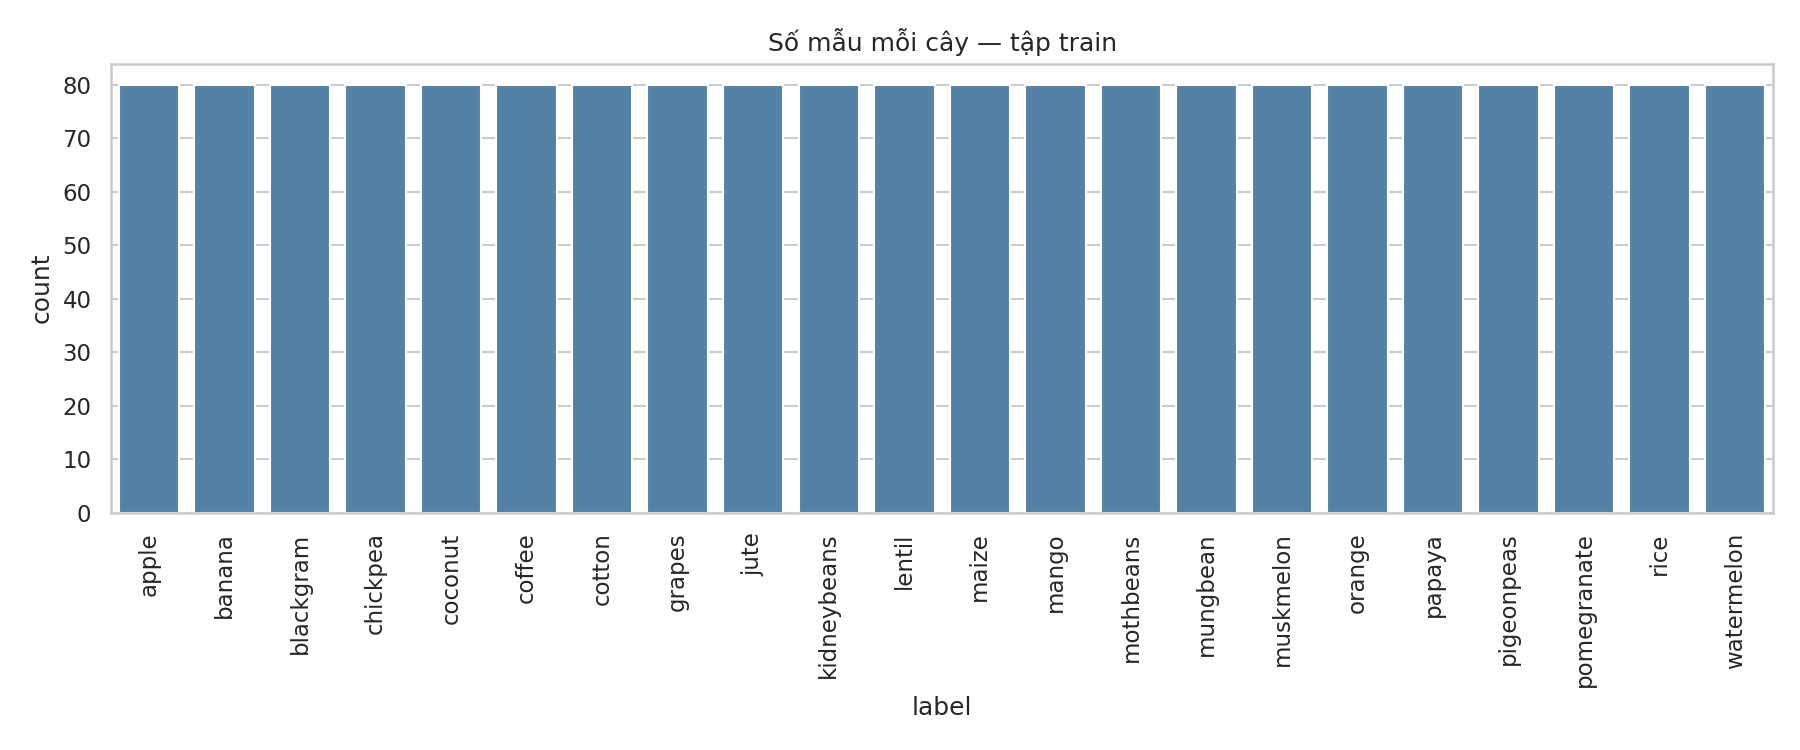
\includegraphics[width=0.98\linewidth,height=0.24\textheight,keepaspectratio]{assets/figure_1.png}

\caption{Phân bố 22 nhãn trên tập huấn luyện}\label{fig:1}\end{figure}


Biểu đồ cho thấy cả 22 lớp đều có 80 mẫu train, nên chưa cần tái lấy mẫu để cân bằng lớp. Nếu kết quả giữa các lớp khác nhau ở giai đoạn sau, cần xem thêm mức chồng lấn đặc trưng và chất lượng nhãn.


\clearpage

\section{2.5. Thống kê mô tả và phân bố đặc trưng}

Các thống kê và hình EDA dưới đây dùng 1.760 mẫu train, không dùng test để lựa chọn cách tiền xử lý. Bảng sau trình bày trung bình, độ lệch chuẩn, trung vị và hai cực trị; các đặc trưng có thang đo khác nhau rõ rệt.


\begingroup
\Needspace{6\baselineskip}
\captionof{table}{Thống kê mô tả trên tập train}\label{tab:5}
\fontsize{11.5}{13.5}\selectfont\setstretch{1.1}
\renewcommand{\arraystretch}{1.15}
\begin{longtable*}{|>{\raggedright\arraybackslash}p{\dimexpr 0.2\linewidth-2\tabcolsep-1.5\arrayrulewidth\relax}|>{\raggedright\arraybackslash}p{\dimexpr 0.16\linewidth-2\tabcolsep-1.5\arrayrulewidth\relax}|>{\raggedright\arraybackslash}p{\dimexpr 0.16\linewidth-2\tabcolsep-1.5\arrayrulewidth\relax}|>{\raggedright\arraybackslash}p{\dimexpr 0.16\linewidth-2\tabcolsep-1.5\arrayrulewidth\relax}|>{\raggedright\arraybackslash}p{\dimexpr 0.16\linewidth-2\tabcolsep-1.5\arrayrulewidth\relax}|>{\raggedright\arraybackslash}p{\dimexpr 0.16\linewidth-2\tabcolsep-1.5\arrayrulewidth\relax}|}
\hline \textbf{Đặc trưng} & \textbf{Trung bình} & \textbf{ĐLC} & \textbf{Min} & \textbf{Trung vị} & \textbf{Max} \\ \hline
\endfirsthead
\hline \textbf{Đặc trưng} & \textbf{Trung bình} & \textbf{ĐLC} & \textbf{Min} & \textbf{Trung vị} & \textbf{Max} \\ \hline
\endhead
N & 50.548 & 36.863 & 0.000 & 37.000 & 140.000 \\ \hline
P & 53.340 & 32.948 & 5.000 & 51.000 & 145.000 \\ \hline
K & 48.143 & 50.709 & 5.000 & 32.000 & 205.000 \\ \hline
temperature & 25.609 & 5.080 & 8.826 & 25.519 & 43.675 \\ \hline
humidity & 71.417 & 22.281 & 14.258 & 80.542 & 99.982 \\ \hline
ph & 6.474 & 0.783 & 3.505 & 6.431 & 9.935 \\ \hline
rainfall & 103.452 & 54.993 & 20.211 & 94.773 & 298.560 \\ \hline
\end{longtable*}
\endgroup


Trên tập train, K có trung vị 32 và giá trị lớn nhất 205; rainfall có trung vị 94,773 và giá trị lớn nhất 298,560. Trong khi đó, ph có trung vị 6,431 và khoảng giá trị nhỏ hơn nhiều. Chênh lệch thang đo có thể khiến một số cột ảnh hưởng mạnh đến khoảng cách giữa hai mẫu. Vì vậy, cần khảo sát chuẩn hóa khi chuẩn bị dữ liệu cho các phương pháp dựa trên khoảng cách.


\begin{figure}[H]\centering

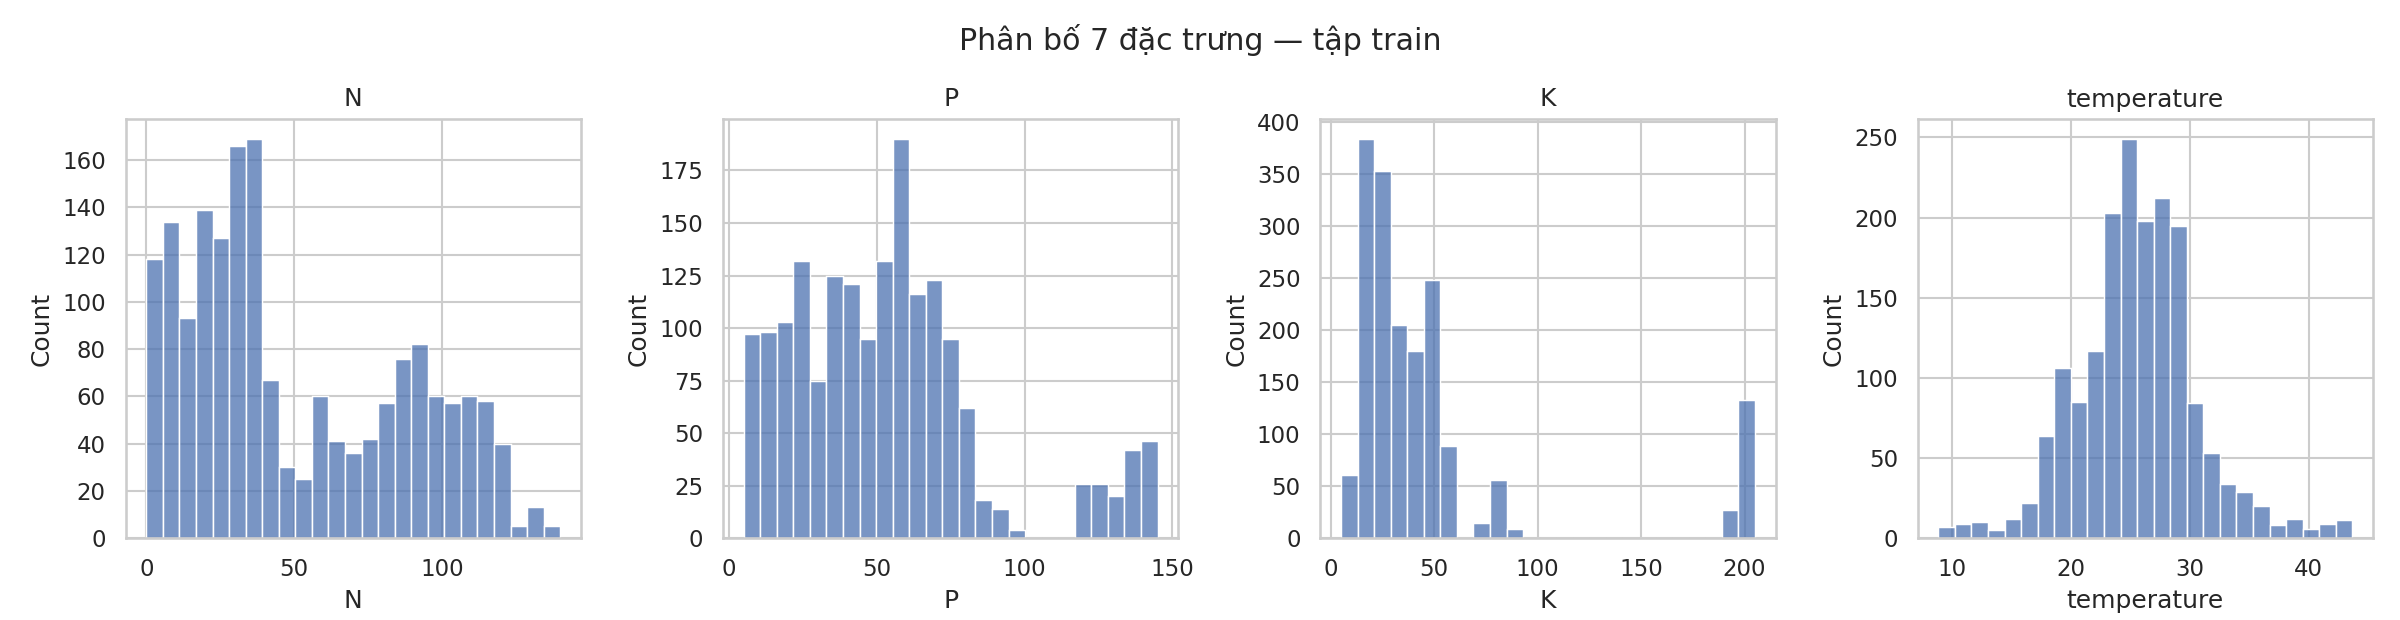
\includegraphics[width=0.98\linewidth,height=0.23\textheight,keepaspectratio]{assets/figure_2.png}

\caption{Phân bố N P K và nhiệt độ trên train}\label{fig:2}\end{figure}


Biểu đồ N và P có nhiều vùng tập trung, thay vì chỉ một đỉnh rõ rệt. Phần lớn giá trị K nằm ở mức thấp, nhưng có thêm một nhóm ở mức cao. Nhiệt độ tập trung quanh vùng giữa và có ít mẫu ở hai đầu. Riêng nhóm K cao cần được xem theo nhãn cây trước khi quyết định giữ hay loại.


\clearpage

\subsection{2.5.1. Độ ẩm pH và lượng mưa}

\begin{figure}[H]\centering

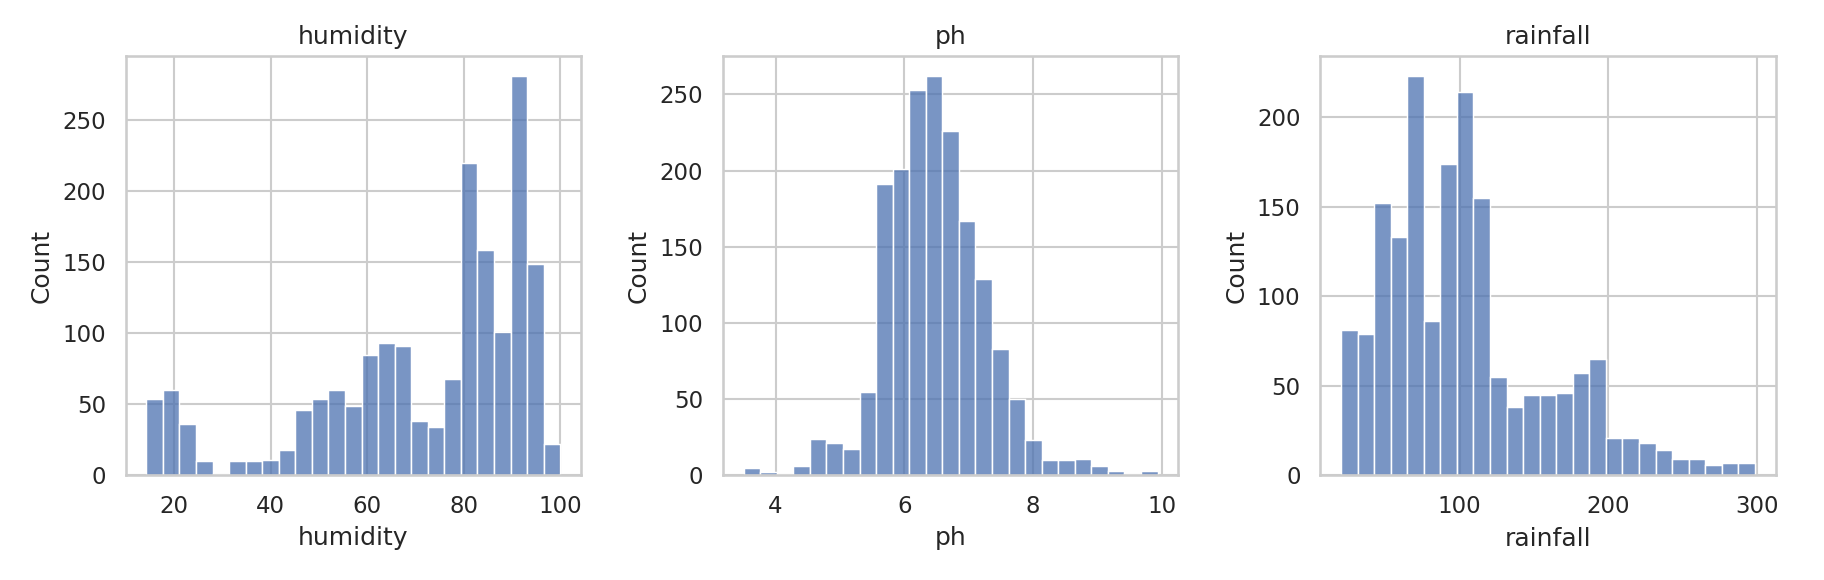
\includegraphics[width=0.98\linewidth,height=0.23\textheight,keepaspectratio]{assets/figure_3.png}

\caption{Phân bố độ ẩm pH và lượng mưa trên train}\label{fig:3}\end{figure}


Độ ẩm có trung bình 71,417\% và trung vị 80,542\%. Biểu đồ cho thấy nhiều mẫu có độ ẩm cao, bên cạnh các nhóm có độ ẩm thấp hơn. pH tập trung chủ yếu quanh 6–7. Lượng mưa có một số giá trị cao tạo thành đuôi lệch phải, làm trung bình lớn hơn trung vị.


Bảy đặc trưng có hình dạng phân bố khác nhau. Do đó, khi kiểm tra các giá trị ở hai đầu, cần xem cả miền hợp lệ và nhãn cây liên quan. Các biểu đồ giúp mô tả bộ dữ liệu và định hướng tiền xử lý; chúng chưa đủ để xác định một ngưỡng canh tác hoặc khẳng định cây sẽ phát triển tốt ngoài thực tế.


\clearpage

\section{2.6. Tương quan và quan hệ với nhãn}

Ma trận Pearson được tính trên bảy cột số của tập train. Cột label chứa tên cây, không có thứ tự lớn nhỏ nên không được chuyển thành số để tính tương quan Pearson với đặc trưng. Quan hệ giữa đặc trưng và nhãn được khảo sát riêng bằng biểu đồ phân bố theo lớp.


\begin{figure}[H]\centering

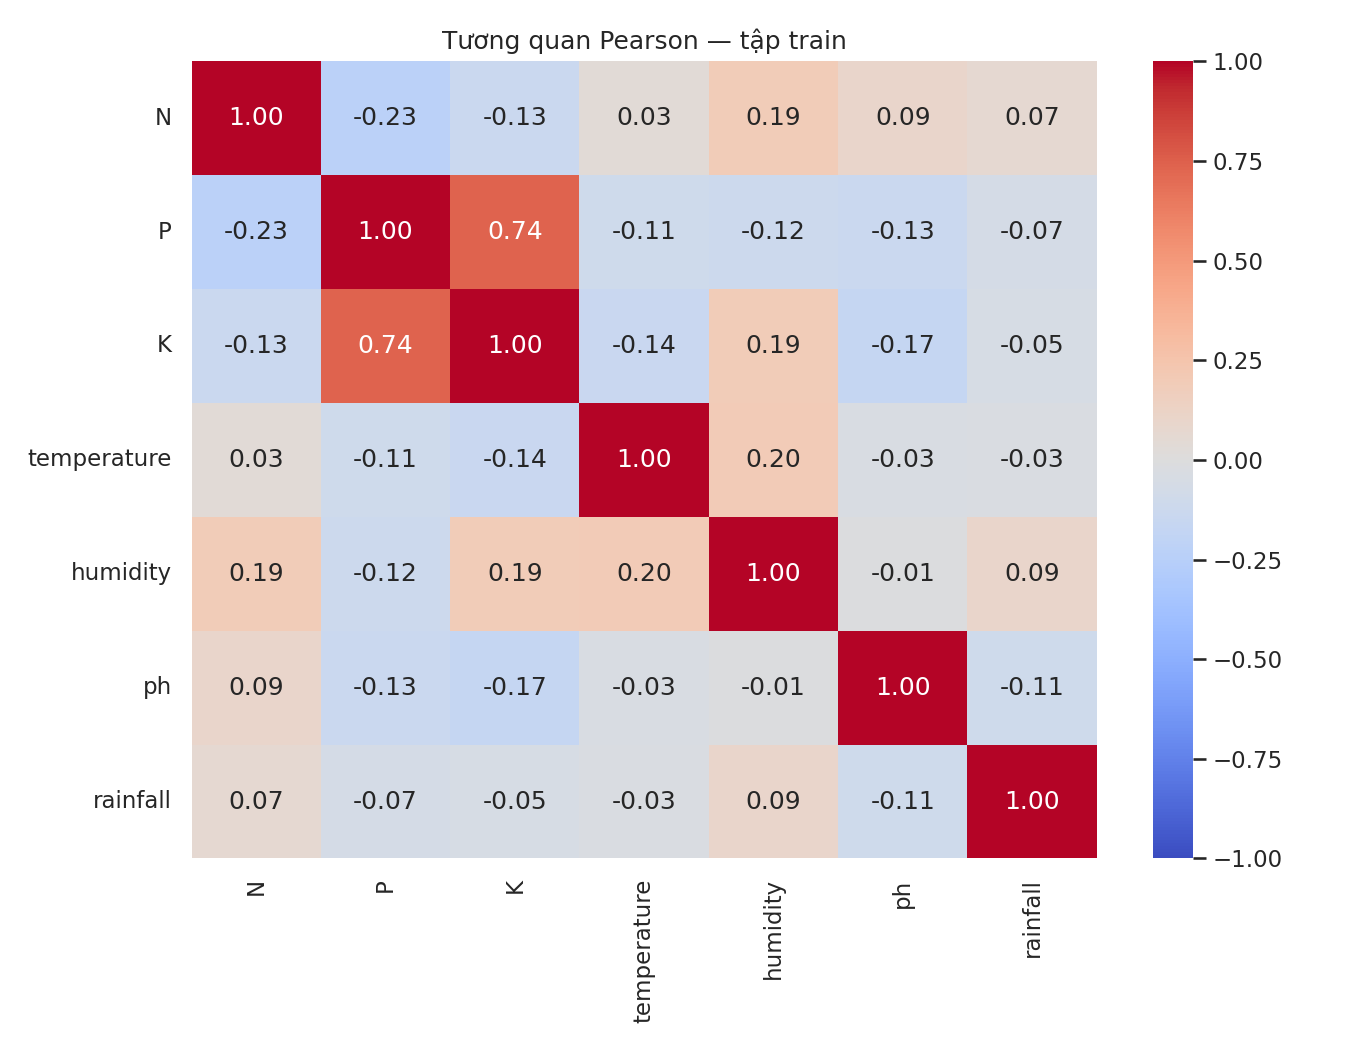
\includegraphics[width=0.98\linewidth,height=0.49\textheight,keepaspectratio]{assets/figure_4.png}

\caption{Tương quan Pearson giữa các đặc trưng train}\label{fig:4}\end{figure}


P và K có hệ số tương quan khoảng 0,736, thể hiện quan hệ tuyến tính rõ hơn phần lớn các cặp còn lại. Lượng mưa có tương quan tuyến tính yếu với các đầu vào khác. Tuy nhiên, ma trận này chưa cho biết trực tiếp mức độ hữu ích của lượng mưa khi phân biệt các nhãn cây.


\clearpage

\subsection{2.6.1. Nhận xét có ý nghĩa cho phương pháp}

P và K có tương quan khoảng 0,736. Hai cột có thể mang một phần thông tin giống nhau, nhưng hiện vẫn được giữ lại. Việc bỏ một cột cần được kiểm tra bằng so sánh kết quả trong cùng điều kiện đánh giá, thay vì chỉ dựa vào hệ số tương quan.


Tương quan giữa rainfall với các cột đầu vào còn lại khá nhỏ. Vì vậy, lượng mưa có thể cung cấp thông tin khác với những biến này. Mức hữu ích cho phân loại cần được đánh giá riêng; tương quan thấp giữa các đầu vào không có nghĩa là một biến không liên quan đến nhãn.


Apple và grapes có giá trị K tập trung ở mức cao hơn nhiều lớp khác. Đây có thể là đặc điểm phân biệt các nhóm cây trong dữ liệu. Vì vậy, các điểm K cao bị đánh dấu bởi IQR được giữ lại để tránh loại mất những mẫu có ý nghĩa đối với phân loại.


Một số lớp có phân bố chồng lấn trên từng đặc trưng. Chẳng hạn, trên biểu đồ K, maize và rice cùng có nhiều giá trị quanh mức 20. Do đó, một mình K khó phân biệt hai nhóm này; cần xét kết hợp với những đặc trưng còn lại.


\begin{figure}[H]\centering

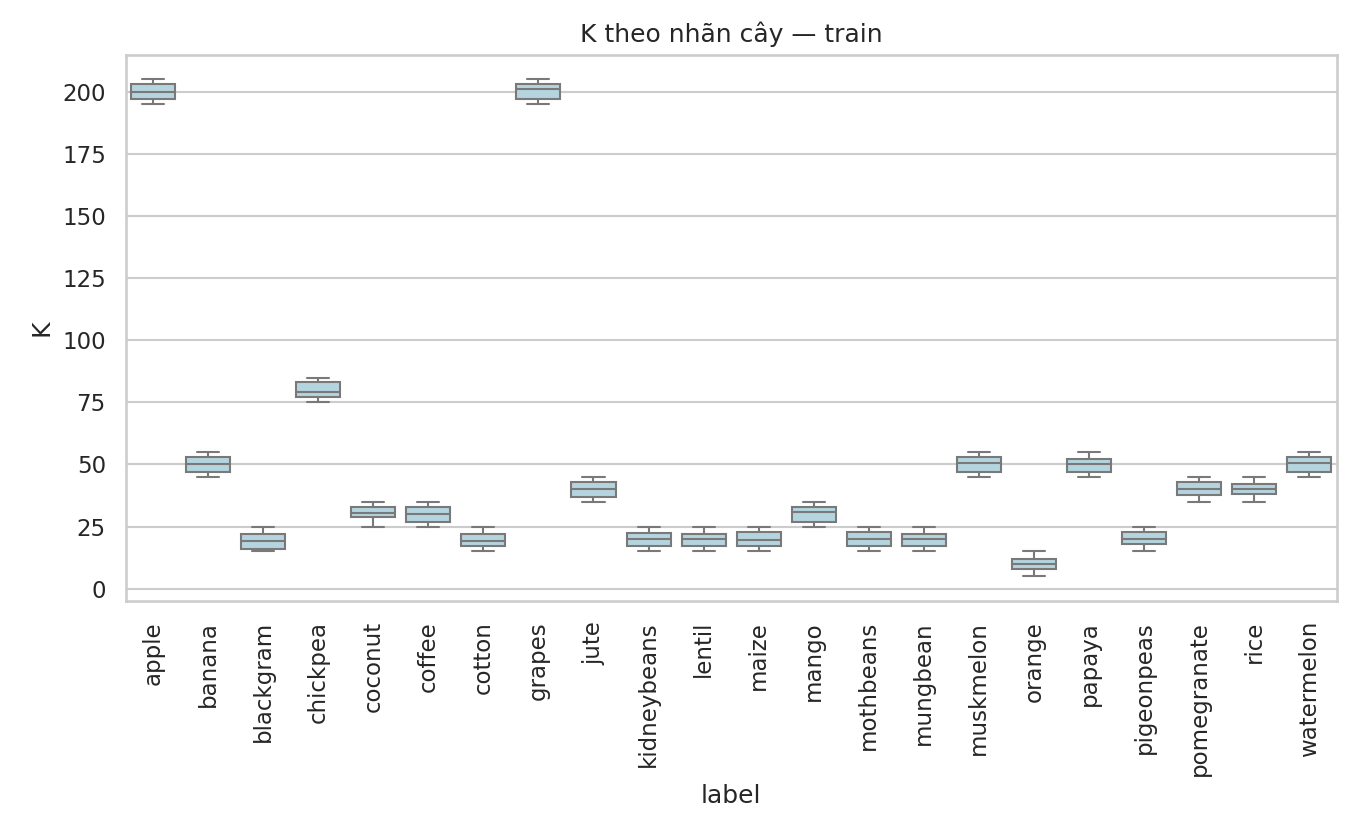
\includegraphics[width=0.98\linewidth,height=0.34\textheight,keepaspectratio]{assets/figure_5.png}

\caption{Phân bố K theo nhãn trên train}\label{fig:5}\end{figure}


Trục ngang thể hiện nhãn cây trồng; trục đứng thể hiện giá trị K theo thang đo của dữ liệu nguồn.


\clearpage

\section{2.7. Định lượng vấn đề chất lượng dữ liệu}

File CSV không có ô thiếu, dòng trùng hoặc nhóm cùng đặc trưng nhưng khác nhãn. Bảy đầu vào đều chuyển được sang số, không có giá trị vô cực. N, P, K, rainfall không âm; humidity thuộc [0,100], ph thuộc [0,14]. Dữ liệu qua được các kiểm tra định dạng và miền giá trị đã đặt ra; độ chính xác của phép đo gốc chưa được xác minh.


\begingroup
\Needspace{6\baselineskip}
\captionof{table}{Vấn đề chất lượng dữ liệu và quyết định xử lý}\label{tab:6}
\fontsize{11.5}{13.5}\selectfont\setstretch{1.1}
\renewcommand{\arraystretch}{1.15}
\begin{longtable*}{|>{\raggedright\arraybackslash}p{\dimexpr 0.26\linewidth-2\tabcolsep-1.5\arrayrulewidth\relax}|>{\raggedright\arraybackslash}p{\dimexpr 0.25\linewidth-2\tabcolsep-1.5\arrayrulewidth\relax}|>{\raggedright\arraybackslash}p{\dimexpr 0.49\linewidth-2\tabcolsep-1.5\arrayrulewidth\relax}|}
\hline \textbf{Vấn đề} & \textbf{Định lượng} & \textbf{Quyết định và lý do} \\ \hline
\endfirsthead
\hline \textbf{Vấn đề} & \textbf{Định lượng} & \textbf{Quyết định và lý do} \\ \hline
\endhead
Thiếu dữ liệu & 0 ô thiếu & Không điền khuyết khi không có giá trị thiếu \\ \hline
Trùng hoàn toàn & 0 dòng & Giữ 2.200 mẫu; vẫn có bước kiểm tra trùng trước chia \\ \hline
Xung đột nhãn theo đặc trưng & 0 nhóm xung đột & Không sửa nhãn bằng suy đoán \\ \hline
Sai định dạng/miền đã kiểm tra & 0 trường hợp & Giữ giá trị; chưa xác minh tính chính xác của thiết bị đo \\ \hline
Mất cân bằng lớp & 100 mẫu/lớp; max/min = 1 & Không oversampling hoặc undersampling \\ \hline
Dấu hiệu ngoại lai IQR trên train & 349/1.760 dòng có ít nhất một cờ & Giữ lại; phân tích theo nhãn trước khi cân nhắc xử lý \\ \hline
Nhóm/địa điểm/thời gian & Không có cột định danh tương ứng & Nêu giới hạn kiểm tra độc lập và rò rỉ theo nhóm \\ \hline
\end{longtable*}
\endgroup


Ngưỡng dưới và ngưỡng trên theo quy tắc 1,5 IQR được tính riêng cho từng đặc trưng trên tập train. Bảng dưới ghi số mẫu nằm ngoài các ngưỡng đó, phục vụ việc kiểm tra những giá trị khác biệt.


\begingroup
\Needspace{6\baselineskip}
\captionof{table}{Số quan sát bị đánh dấu theo quy tắc 1,5 IQR trên train}\label{tab:7}
\fontsize{11.5}{13.5}\selectfont\setstretch{1.1}
\renewcommand{\arraystretch}{1.15}
\begin{longtable*}{|>{\raggedright\arraybackslash}p{\dimexpr 0.4\linewidth-2\tabcolsep-1.5\arrayrulewidth\relax}|>{\raggedright\arraybackslash}p{\dimexpr 0.25\linewidth-2\tabcolsep-1.5\arrayrulewidth\relax}|>{\raggedright\arraybackslash}p{\dimexpr 0.35\linewidth-2\tabcolsep-1.5\arrayrulewidth\relax}|}
\hline \textbf{Đặc trưng} & \textbf{Số mẫu} & \textbf{Tỷ lệ trên train} \\ \hline
\endfirsthead
\hline \textbf{Đặc trưng} & \textbf{Số mẫu} & \textbf{Tỷ lệ trên train} \\ \hline
\endhead
N & 0 & 0.00\% \\ \hline
P & 108 & 6.14\% \\ \hline
K & 160 & 9.09\% \\ \hline
temperature & 72 & 4.09\% \\ \hline
humidity & 24 & 1.36\% \\ \hline
ph & 43 & 2.44\% \\ \hline
rainfall & 82 & 4.66\% \\ \hline
\end{longtable*}
\endgroup


Có 349 mẫu train ngoài ngưỡng IQR ở ít nhất một cột, chiếm 19,83\%. Một mẫu có thể bị đánh dấu ở nhiều cột. Các mẫu được giữ lại vì chưa có bằng chứng cho thấy đó là dữ liệu sai.


\section{2.8. Tiền xử lý và so sánh trước sau}

Bước đọc dữ liệu kiểm tra tên cột, chuyển đặc trưng sang số, thống nhất cách viết nhãn và kiểm tra giá trị hợp lệ. Quy tắc loại dòng trùng hoàn toàn được đặt trước bước chia tập; với file hiện tại, không có dòng nào bị loại. Nhãn cây được giữ ở dạng chuỗi vì thư viện phân loại hỗ trợ trực tiếp dạng này.


Phần mã chuẩn bị cho giai đoạn mô hình có ba lựa chọn: giữ nguyên thang đo, StandardScaler và MinMaxScaler. Bộ chuẩn hóa được đặt trong Pipeline để chỉ fit trên phần train của mỗi fold, sau đó áp dụng cho validation hoặc test. Các ô này chưa được chạy trong lần thực hiện Bài kiểm tra 1, nên báo cáo chưa có kết quả so sánh chuẩn hóa.


\begingroup
\Needspace{6\baselineskip}
\captionof{table}{Dữ liệu trước và sau kiểm tra làm sạch}\label{tab:8}
\fontsize{11.5}{13.5}\selectfont\setstretch{1.1}
\renewcommand{\arraystretch}{1.15}
\begin{longtable*}{|>{\raggedright\arraybackslash}p{\dimexpr 0.48\linewidth-2\tabcolsep-1.5\arrayrulewidth\relax}|>{\raggedright\arraybackslash}p{\dimexpr 0.26\linewidth-2\tabcolsep-1.5\arrayrulewidth\relax}|>{\raggedright\arraybackslash}p{\dimexpr 0.26\linewidth-2\tabcolsep-1.5\arrayrulewidth\relax}|}
\hline \textbf{Thuộc tính} & \textbf{Trước} & \textbf{Sau} \\ \hline
\endfirsthead
\hline \textbf{Thuộc tính} & \textbf{Trước} & \textbf{Sau} \\ \hline
\endhead
Số mẫu & 2200 & 2200 \\ \hline
Số đặc trưng đầu vào & 7 & 7 \\ \hline
Số nhãn & 22 & 22 \\ \hline
Giá trị thiếu & 0 & 0 \\ \hline
Dòng trùng hoàn toàn & 0 & 0 \\ \hline
Số mẫu mỗi lớp & 100 & 100 \\ \hline
Điểm IQR bị xóa & \rule{0pt}{15pt} & 0 \\ \hline
\end{longtable*}
\endgroup


Sau kiểm tra, dữ liệu vẫn gồm 2.200 mẫu vì không có ô thiếu hoặc dòng trùng. Các điểm ngoài ngưỡng IQR được giữ lại vì có thể phản ánh đặc điểm riêng của từng loại cây.


\section{2.9. Chia dữ liệu và lý giải chỉ số đánh giá}

Dữ liệu được chia phân tầng theo label với tỷ lệ train/test là 80/20 và random\_state=42. Kết quả có 1.760 mẫu train và 440 mẫu test. Tập train tiếp tục được chia sẵn thành 5 fold phân tầng. Mỗi lượt có 1.408 mẫu dùng để học và 352 mẫu validation, tương ứng 64 và 16 mẫu mỗi lớp. Các fold được lưu để những phương pháp ở giai đoạn sau dùng cùng cách chia.


Kiểm định chéo phân tầng được chọn để mỗi lượt đều có đủ 22 lớp và giữ cùng tỷ lệ nhãn. F1 macro là chỉ số chính vì tính kết quả cho từng lớp với trọng số ngang nhau; Accuracy bổ sung tỷ lệ dự đoán đúng toàn bộ. Dự kiến báo cáo trung bình và độ lệch chuẩn qua 5 fold, sau đó đánh giá trên test khi đã chọn xong cấu hình. Dữ liệu không có mã thửa ruộng hoặc thời gian nên chưa thể chia theo các nhóm này.


\section{2.10. Lựa chọn thuật toán}

\emptyspace

\section{2.11. Mô hình cơ sở}

\emptyspace

\section{2.12. Quy trình huấn luyện và cài đặt mô hình}

\emptyspace

\majorheading{CHƯƠNG 3. THỬ NGHIỆM VÀ ĐÁNH GIÁ}

\section{3.1. Thiết lập thực nghiệm}

\emptyspace

\section{3.2. Kết quả huấn luyện và kiểm định chéo}

\emptyspace

\section{3.3. Đánh giá trên tập kiểm tra và so sánh với mô hình cơ sở}

\emptyspace

\section{3.4. Phân tích lỗi và khả năng khái quát hóa}

\emptyspace

\section{3.5. Cải tiến và so sánh}

\emptyspace

\section{3.6. Chương trình minh họa}

\emptyspace

\section{3.7. Kết luận và hướng phát triển}

\emptyspace

\majorheading{TÀI LIỆU THAM KHẢO}

{\setstretch{1.1}\noindent [1] G. James, D. Witten, T. Hastie, R. Tibshirani và J. Taylor (2023), An Introduction to Statistical Learning with Applications in Python, Springer. Trang tác giả: \url{https://www.statlearning.com/}.\par}\vspace{6pt}

{\setstretch{1.1}\noindent [2] Scikit-learn developers, Imputation of missing values, tài liệu phiên bản 1.7. \url{https://scikit-learn.org/1.7/modules/impute.html}.\par}\vspace{6pt}

{\setstretch{1.1}\noindent [3] Scikit-learn developers, Preprocessing data. \url{https://scikit-learn.org/1.7/modules/preprocessing.html}.\par}\vspace{6pt}

{\setstretch{1.1}\noindent [4] Scikit-learn developers, Feature selection. \url{https://scikit-learn.org/1.7/modules/feature_selection.html}.\par}\vspace{6pt}

{\setstretch{1.1}\noindent [5] Scikit-learn developers, Cross-validation: evaluating estimator performance. \url{https://scikit-learn.org/1.7/modules/cross_validation.html}.\par}\vspace{6pt}

{\setstretch{1.1}\noindent [6] Scikit-learn developers, Validation curves: plotting scores to evaluate models. \url{https://scikit-learn.org/1.7/modules/learning_curve.html}.\par}\vspace{6pt}

{\setstretch{1.1}\noindent [7] Scikit-learn developers, Metrics and scoring: quantifying the quality of predictions. \url{https://scikit-learn.org/1.7/modules/model_evaluation.html}.\par}\vspace{6pt}

{\setstretch{1.1}\noindent [8] Scikit-learn developers, Common pitfalls and recommended practices. \url{https://scikit-learn.org/1.7/common_pitfalls.html}.\par}\vspace{6pt}

{\setstretch{1.1}\noindent [9] Atharva Ingle, Crop Recommendation Dataset, Kaggle. \url{https://www.kaggle.com/datasets/atharvaingle/crop-recommendation-dataset}. Metadata: \url{https://www.kaggle.com/api/v1/datasets/view/atharvaingle/crop-recommendation-dataset} (25/10/2026).\par}\vspace{6pt}
